% Example definitions.
% --------------------
\section{Dimensionality reduction for vowel space}
IST has studied the possibility of reducing the dimensionality of the
motor space for the production of vowels. The study is motivated by results on Linguistics and
Phonetics, where the vowel space in represented is motor terms in a 2D
representation. We show that a 2-dimensional plane generated by the
convex combination of 3 extremal motor primitives is able to
adequately represent the vowel acoustic space, allowing for simple and
efficient learning and classification methods. An additional advantage
is that, since the synthesis is based on two sole parameters, it is
easy and intuitive to graphically visualize the motor-to-acoustic
manifold, allowing a better characterization of its properties. 

\begin{figure}[!h]
  \centering
\begin{tabular}{cc}
%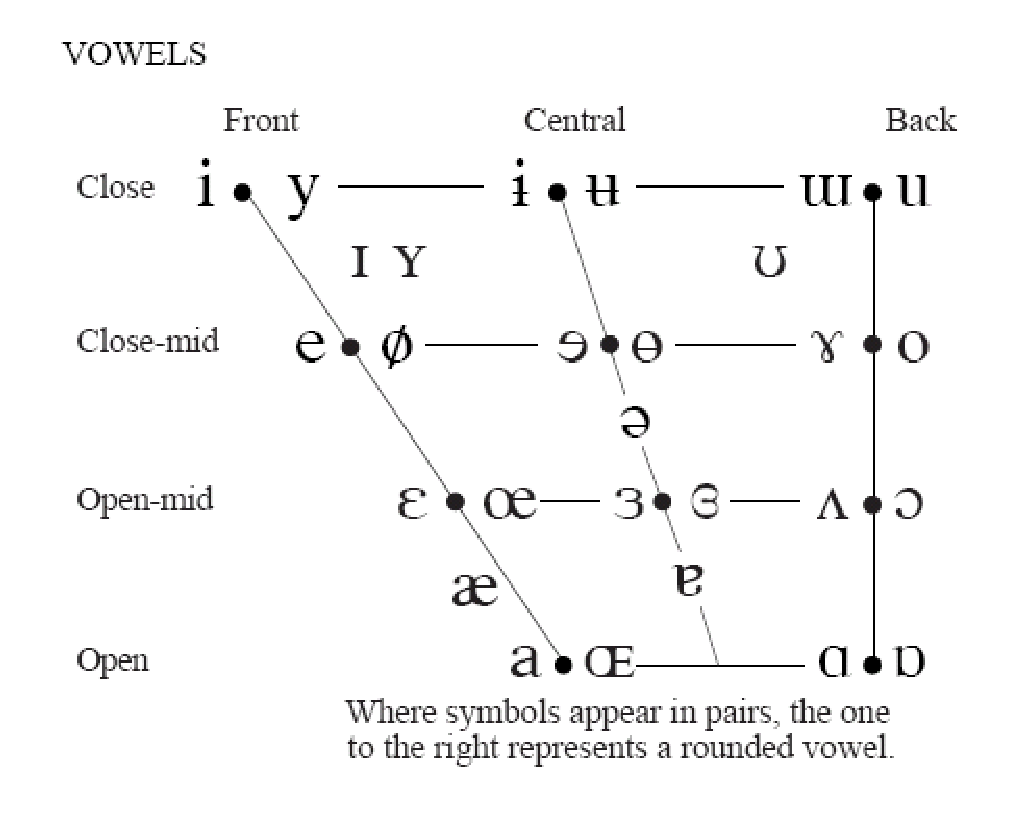
\includegraphics[width=0.45\textwidth]{include/vowels/images/vowels}} &
%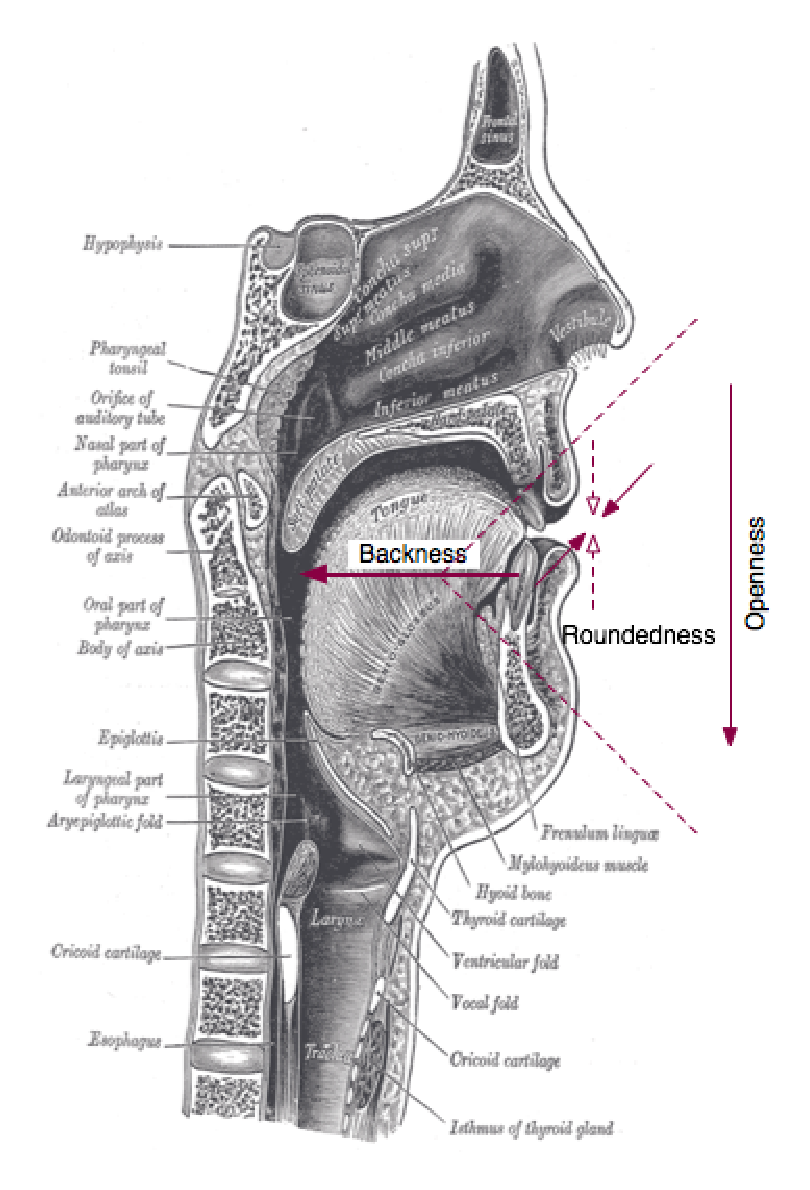
\includegraphics[width=0.45\textwidth]{include/vowels/images/vtdiag}} \\
(a) & (b) \\
\end{tabular}
\caption{Articulatory degrees of freedom in the IPA chart
  representation: (a) International Phonetic Alphabet chart for oral
  vowels. (b) Main degrees of freedom represented in the IPA chart.}
\label{fig:ipavowels}
\end{figure}

The schematic in the International Phonetic Alphabet (IPA) for oral
vowels in Figure \ref{fig:ipavowels}(a) shows the distribution of
vocalic sounds in three dimensions relative to the human vocal tract:
height (vertical axis), backness (horizontal axis) and roundedness
(lip rounding) \cite{IPA} as illustrated.
 
This choice of reference frame has roots in the physiology of the
phonatory system. The vocal tract configuration for oral vowels is
function of the tongue, the jaw and the lips. The jaw and lips can
have several degrees of openness, the tongue can assume the
articulatory positions in front, center or back of the oral cavity and
the lips can also change the vocal tract by rounding. So, these three
articulatory parameters are considered the main degrees of freedom of
vocalic speech sounds, the directions that better explain the
inter-vowel variation. Nevertheless, there are other articulatory
parameters that influence vowel quality, although they are not
determinant in most spoken languages.

In most languages, rounded and unrounded vowels are not minimal pairs,
i.e., for the same articulatory configuration, roundedness does not
create two different phonological vowels. For this reason, the main
articulatory dimensions for vocalic sounds in the human vocal tract
are the height and backness, motivating the approximation proposed in
this paper --- whatever the dimensionality of the articulatory space
we consider, there is an two-dimensional subspace approximation that
maps the vowel system of most languages.
The phones  \textipa{[i]}, \textipa{[a]} and \textipa{[u]} define a
set of axis in the 2D plane of the articulatory parameters of
\emph{height} and \emph{backness}. These three vowels are called
\emph{corner vowels} because they represent extreme placements of the
tongue forming the corners of a triangle in articulatory space. They
also form a triangle in formant space (F1 --
F2)\cite{TITZE}. Therefore, we consider these phones the extremal
points in our model, and will produce the remaining ones by their
convex combination. This will be detailed in the following Section.

\subsection{The Speech Production Model}
To test and validate our proposal we use a known articulatory speech
synthesizer. This will allow us to do systematic tests and quantify
the errors arising from the proposed approximation. From realizations
of the extremal phones \textipa{[i]}, \textipa{[a]} and \textipa{[u]},
we generate a dense representation of the feasible acoustic
signals. Then, to evaluate the model, we compute the acoustic errors
outside the feasible set.

\subsubsection{Articulatory Synthesizer}
The synthesizer in use\footnote{Available at the CNS Speech Lab
  webpage \texttt{http://speechlab.bu.edu/VTCalcs.php}} is a Matlab
version of Shinji Maeda's Vocal Tract Calculator (\emph{VTCalcs})
\cite{MAEDA}. The 7 articulatory parameters are \emph{jaw, tongue,
  shape, apex, lip\_ht} (lip hight), \emph{lip\_pr}, (lip protrusion),
\emph{larynx}. Each one can assume any value in $[-3;3]$. The
articulator parameters are presumed independent, which is not the
case, leading sometimes to improbable configurations of the vocal
tract, producing a non human or even no sound.
The space of the articulators in  \emph{VTCalcs} is homographic to
$\mathds{R}^{7}$, but to produce vocalic voiced sounds only 6
parameters are distinctive, since larynx controls the voicing. The
synthesizer's output is a sound represented by its temporal
amplitude. To analyze the sound waveform we use the Mel Frequency
Cepstral Coefficients (MFCC) \cite{Davis80}, using $12$ coefficients.

Let vector $\mathbf{v} \in \mathcal{V} \subset \mathds{R}^{6}$
represent a configuration of the six-dimensional synthesizer's
articulatory space and  $\mathbf{a} \in \mathcal{A} \subset
\mathds{R}^{12} $ be a vector of MFCC coefficients in the acoustic
space. We define the synthesis function as:
\begin{equation}
f : \mathcal{V} \mapsto \mathcal{A}, \quad \mathbf{a} = f( \mathbf{v})
\end{equation}
This is a complicated function to work with because it is not
invertible -- distinct articulatory configurations may lead to very
similar sounds (in particular, many configurations generate no sound
at all). Therefore, there is ambiguity in the identification of motor
configurations corresponding to the listened acoustic signals, which
may pose problems to motor-based learning and recognition
algorithms. To deal with this we define a subspace of $\mathcal{V}$
where the restriction of $f$ to this subspace is invertible.

\subsubsection{Dimensionality Reduction}
According to Linguistics and
Phonetics knowledge, most of the vowel production capabilities of the
human vocal tract can be explained by two parameters related to the
height and backness of the articulators. Therefore, we will define a
two-dimensional subspace of the full articulatory space, generated by
a convex combination of vowels corresponding to extremal positions in
the articulatory space.

Considering the $\mathds{R}^{6}$ prototypes included in \emph{VTCalcs}
for the phones \textipa{[i]},\textipa{[a]} and \textipa{[u]}, it is
possible to generate an affine space with all the properties of a
convex space. Let  $a_{0}, u_{0}$ and $i_{0} \ \in  \mathds{R}^6$ be
the \emph{VTCalcs}  vowel prototypes for \textipa{[i]}, \textipa{[u]}
and \textipa{[a]}
and a two-dimensional vector $\mathbf{p} \in \mathcal{V} : \mathbf{p} = (\alpha, \beta)$, with $\alpha$ and $\beta$ real parameters.
A convex combination of the given points forming a 2-dimensional
triangle, can be defined by the function:
\begin{eqnarray*}
 & v : \mathcal{P} \subset \mathds{R}^2 \mapsto \mathcal{M} \subset \mathcal{V} \\
 & v(\alpha, \beta) = \alpha\  i_{0}+\beta\  a_{0}+ (1-\alpha-\beta) \ u_{0}
\end{eqnarray*}
where the input space $\cal P$ is defined as:
\begin{equation*}
\mathcal{P} = \left\{ (\alpha, \beta) : \alpha + \beta \leq 1  \land  \alpha , \beta \geq 0 \right\}
\end{equation*}

Let us denote $\mathcal{M}$ be the image of $v$, and call it the
\textit{Motor Space}. We define function $f_2$ as the restriction of
the synthesizer's function $f$ to the motor space:
\begin{equation}
f_2 : \mathcal{M} \mapsto \mathcal{A}_2 \subset \mathcal{A}
\end{equation} 
We will denote $f_2$ as the \textit{Motor-Acoustic Map}. The image of
this function will produce a 2D manifold $\mathcal{A}_2$ in the MFCC
acoustic space. Given the choice of the \textit{Motor-Space} and the
properties of the used synthesizer, $f_2$ is invertible and the
inverse $f_{2}^{-1}$ is an acoustic to motor map. A schematic
representation of the proposed vowel production model is shown in
Figure \ref{fig:diagram}.
\begin{figure}[!ht]
  \centering
  %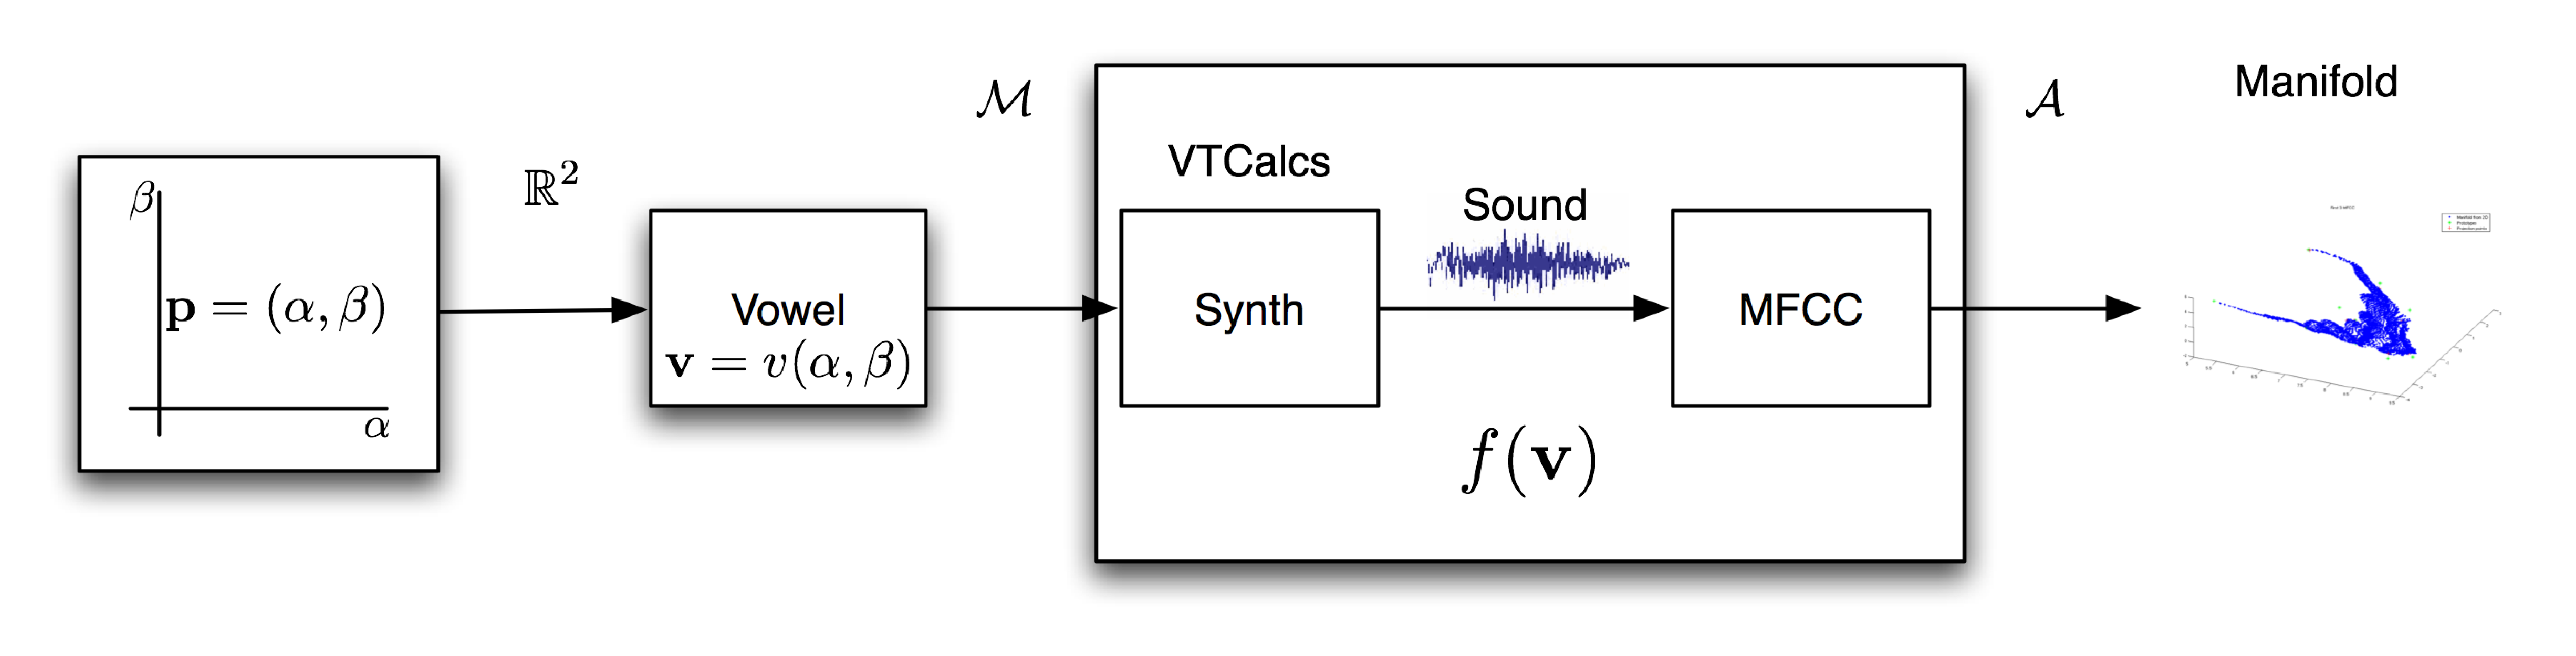
\includegraphics[width=85mm]{include/vowels/images/diagram}
  \caption{Vowel generation diagram.}
  \label{fig:diagram}
\end{figure}

To graphically illustrate the \textit{acoustic manifold}
$\mathcal{A}_2$ we have sampled the parameter space $\mathcal{P}$ in
steps of $0.01$ in the $\alpha$ and $\beta$ parameters, generating a
discrete set of 5000 samples:
\begin{equation*}
\mathcal{P}_d = \left\{ \mathbf{p}_i,\ i \in 1 \cdots 5000 \right\}
\end{equation*} 
These samples were then used to generate a motor-space sample set,
using function $v$:
\begin{equation*}
\mathcal{M}_d = \left\{ \mathbf{m}_i = v(\mathbf{m}_i),\  i \in 1 \cdots 5000 \right\}
\end{equation*} 
Thus a discrete sampling of the acoustic manifold was created using
the synthesizer's function:
\begin{equation}
\mathcal{A}_{2d} = \left\{ \mathbf{a}_i = f_2(\mathbf{m}_i), \ i \in 1 \cdots 5000 \right\}
\label{eq:manif}
\end{equation} 
The first three coordinates of the sampled acoustic manifold are
plotted in Figure \ref{fig:manif}.
\begin{figure}[!h]
\hspace{-1cm}
%  \centering
  %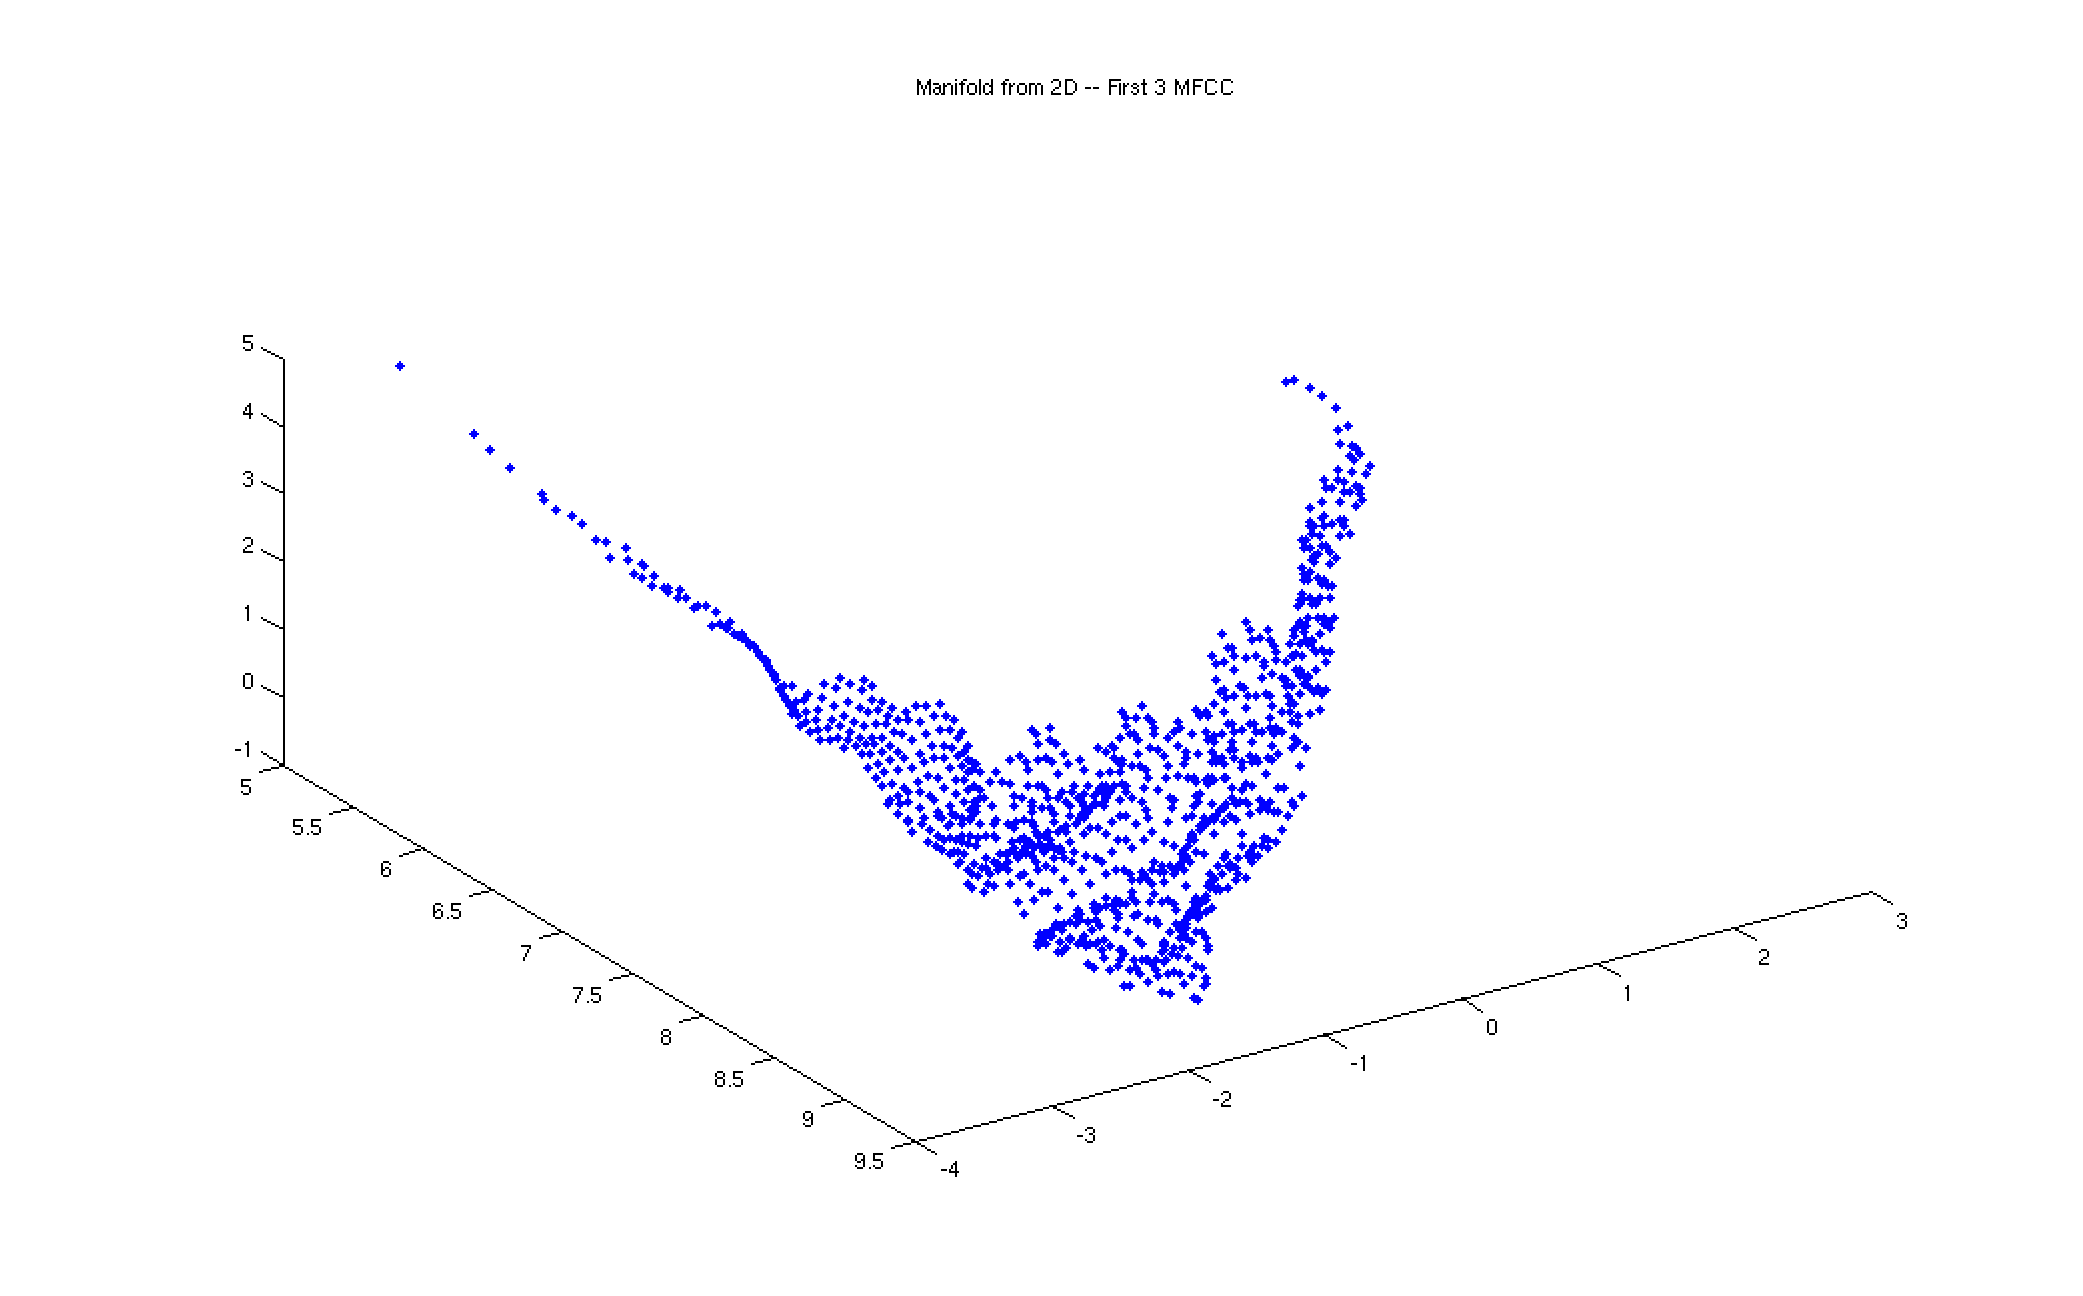
\includegraphics[width=95mm]{include/vowels/images/manifold}
  \caption{Representation of the first three Mel coefficients of the
    acoustic manifold.}
  \label{fig:manif}
\end{figure}

\subsection{Experimental Results}
To validate the proposed model we compute the acoustic errors produced
by the MFCC coefficients of arbitrary test vowels $\mathbf{a}^t$, by
computing the euclidean distance to their projection onto the acoustic
manifold. We also consider the errors produced by the $f$ domain
restriction to $\mathcal{M}$. Since we do not have a analytic
expression for the manifold, we use its sampled version defined in
(\ref{eq:manif}). To compute the projection we use the nearest
neighbor operator:

\begin{equation}
nn(\mathbf{a}^{t} ) = \left\{ \mathbf{a}_{i} \in \mathcal{A}_{2d} : i = \argmin_{i}\left\{ \| \mathbf{a}_{i} - \mathbf{a}^{t} \|_{2}\right\} \right\}
\end{equation}
The approximation error is then computed by:
\begin{equation}
E(\mathbf{a}^{t} ) = \| \mathbf{a}^{t} - nn(\mathbf{a}^{t}) \|_{2}
\end{equation}
The relative error is given by
\begin{equation}
\delta(\mathbf{a}^{t} ) = \frac{E(\mathbf{a}^{t} ) }{Area(\mathcal{A}_{2d} ) } \  100\% 
\end{equation}

The area of $\mathcal{A}_{2d}$ was measured through \emph{geodesic paths} along the manifold, determined with the Isomap algorithm as described in \cite{Tenenbaum00}. 

\subsubsection{Effects of dimensionality reduction}
It was determined through Isomap the dimensionality of the image of $f$, with a residual variance of 0.197.

\begin{figure}[!h]
%\hspace{-1cm}
 \centering
  %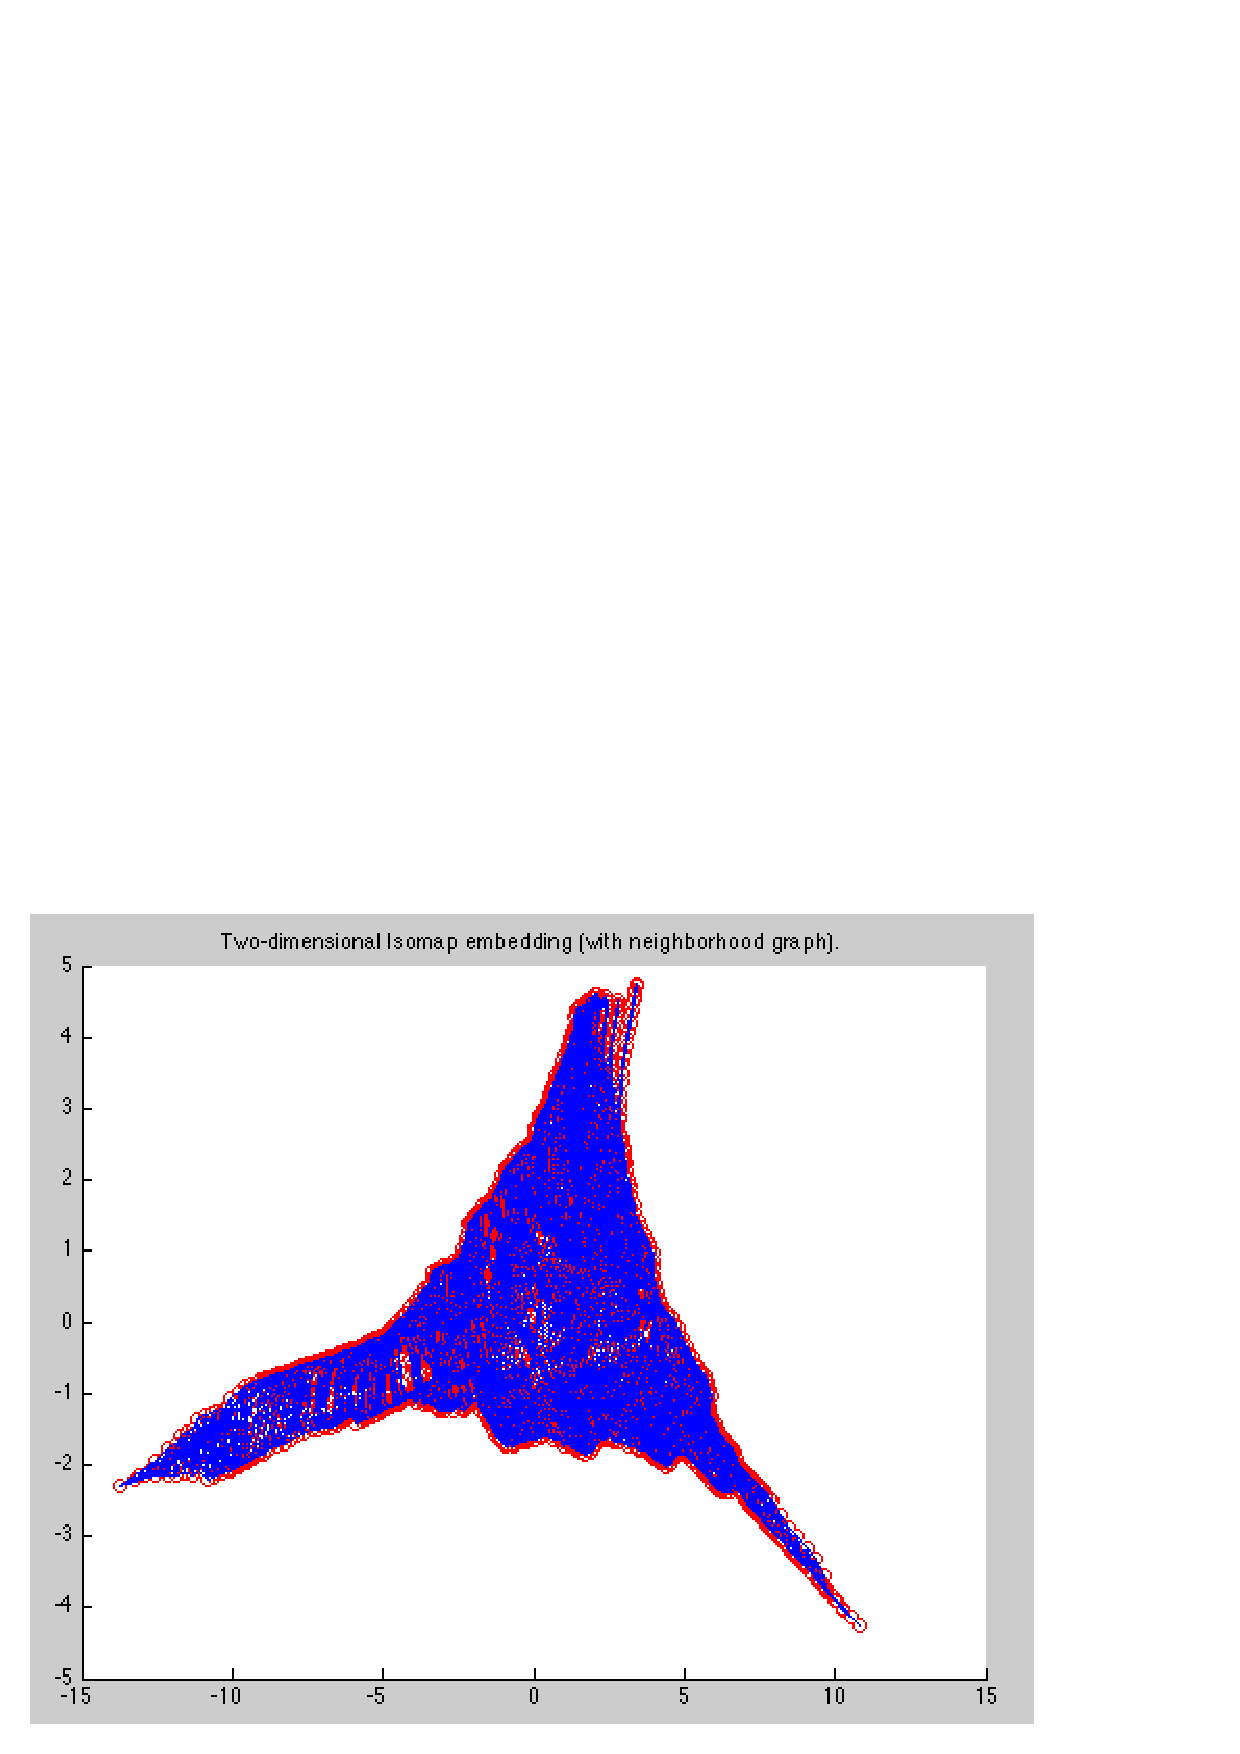
\includegraphics[width=0.4\textwidth]{include/vowels/images/isomap2d.png}
  \caption{Isomap embedding for the 2-dimensional manifold $\mathcal{A}_{2d}$.}
  \label{fig:isomap2D}
\end{figure}

\subsection{Vowel prototypes}
In the \emph{VTCalcs} matlab package there are 11 prototypes for oral
vowels that were used to evaluate the amount of error introduced in
the 2-dimensional approximation. The error was measured as described
above, and the results are shown in Table \ref{table:convexmaeda}. Six
portuguese prototype vowels were also used. The quadratic error is
shown in Table \ref{table:convexpt}.
\begin{table} [t,h]
\caption{\label{table:convexmaeda} {\it Approximation error for the chosen \emph{VTCalcs} prototypes.}}
\vspace{2mm}
\centerline{
\begin{tabular}{|c|c|c|c|}
\hline
vowel & symbol & quadratic error & relative error (\%) \\
\hline  \hline
1 & iy &  0.0009 &   0.3460\\ 
2  & ey & 0.0101 &    1.1827\\
3  &eh& 0.0321 &    2.0431\\
4  & ah & 0.2297 &   5.0325\\
5  & aa&  0.0734 &   2.7715\\
6  & ao&1.6727 &   14.0579\\
7  & oh& 2.7736 &   19.5274\\
8  & uw& 0.0024 &    0.7372\\
9  & iw& 2.1443  &  18.4749\\
10 & ew&  0.0704 &     3.2427\\
11 & oe&   0.0194 &     1.5963\\
\hline
\end{tabular}}
\label{tab:proto}
\end{table}
\begin{table} [t,h]
\caption{\label{table:convexpt} {\it Approximation error for the chosen portuguese prototypes.}}
\vspace{2mm}
\centerline{
\begin{tabular}{|c|c|c|}
\hline
phone & quadratic error \\
\hline  \hline
\textipa{1}&    0.0044\\
\textipa{5}&      1.6649\\
 \textipa{E}&     0.1434\\
\textopeno&      1.6699\\
\textipa{e}&      1.1169\\
 \textipa{o}&     2.8640\\
 a & 0.0734\\
 u & 0.0024 \\
 i & 0.0009\\
 \hline
\end{tabular}}
\label{tab:proto}
\end{table}

These errors are graphically illustrated in Figure \ref{fig:convport},
where the first three MFCC coefficients of the test vowels are plotted
together with the acoustic manifold. The average approximation error
is about $6\%$. Vowels $6$, $7$, and $9$ present larger relative
errors (about $20\%$), but acoustically they are hardly
distinguishable from their projection. This could reveal some
limitations in the sound representation via MFCC's that we will
address in future work.

\begin{figure}[!h]
  %\centering
  \hspace{-1cm}
  %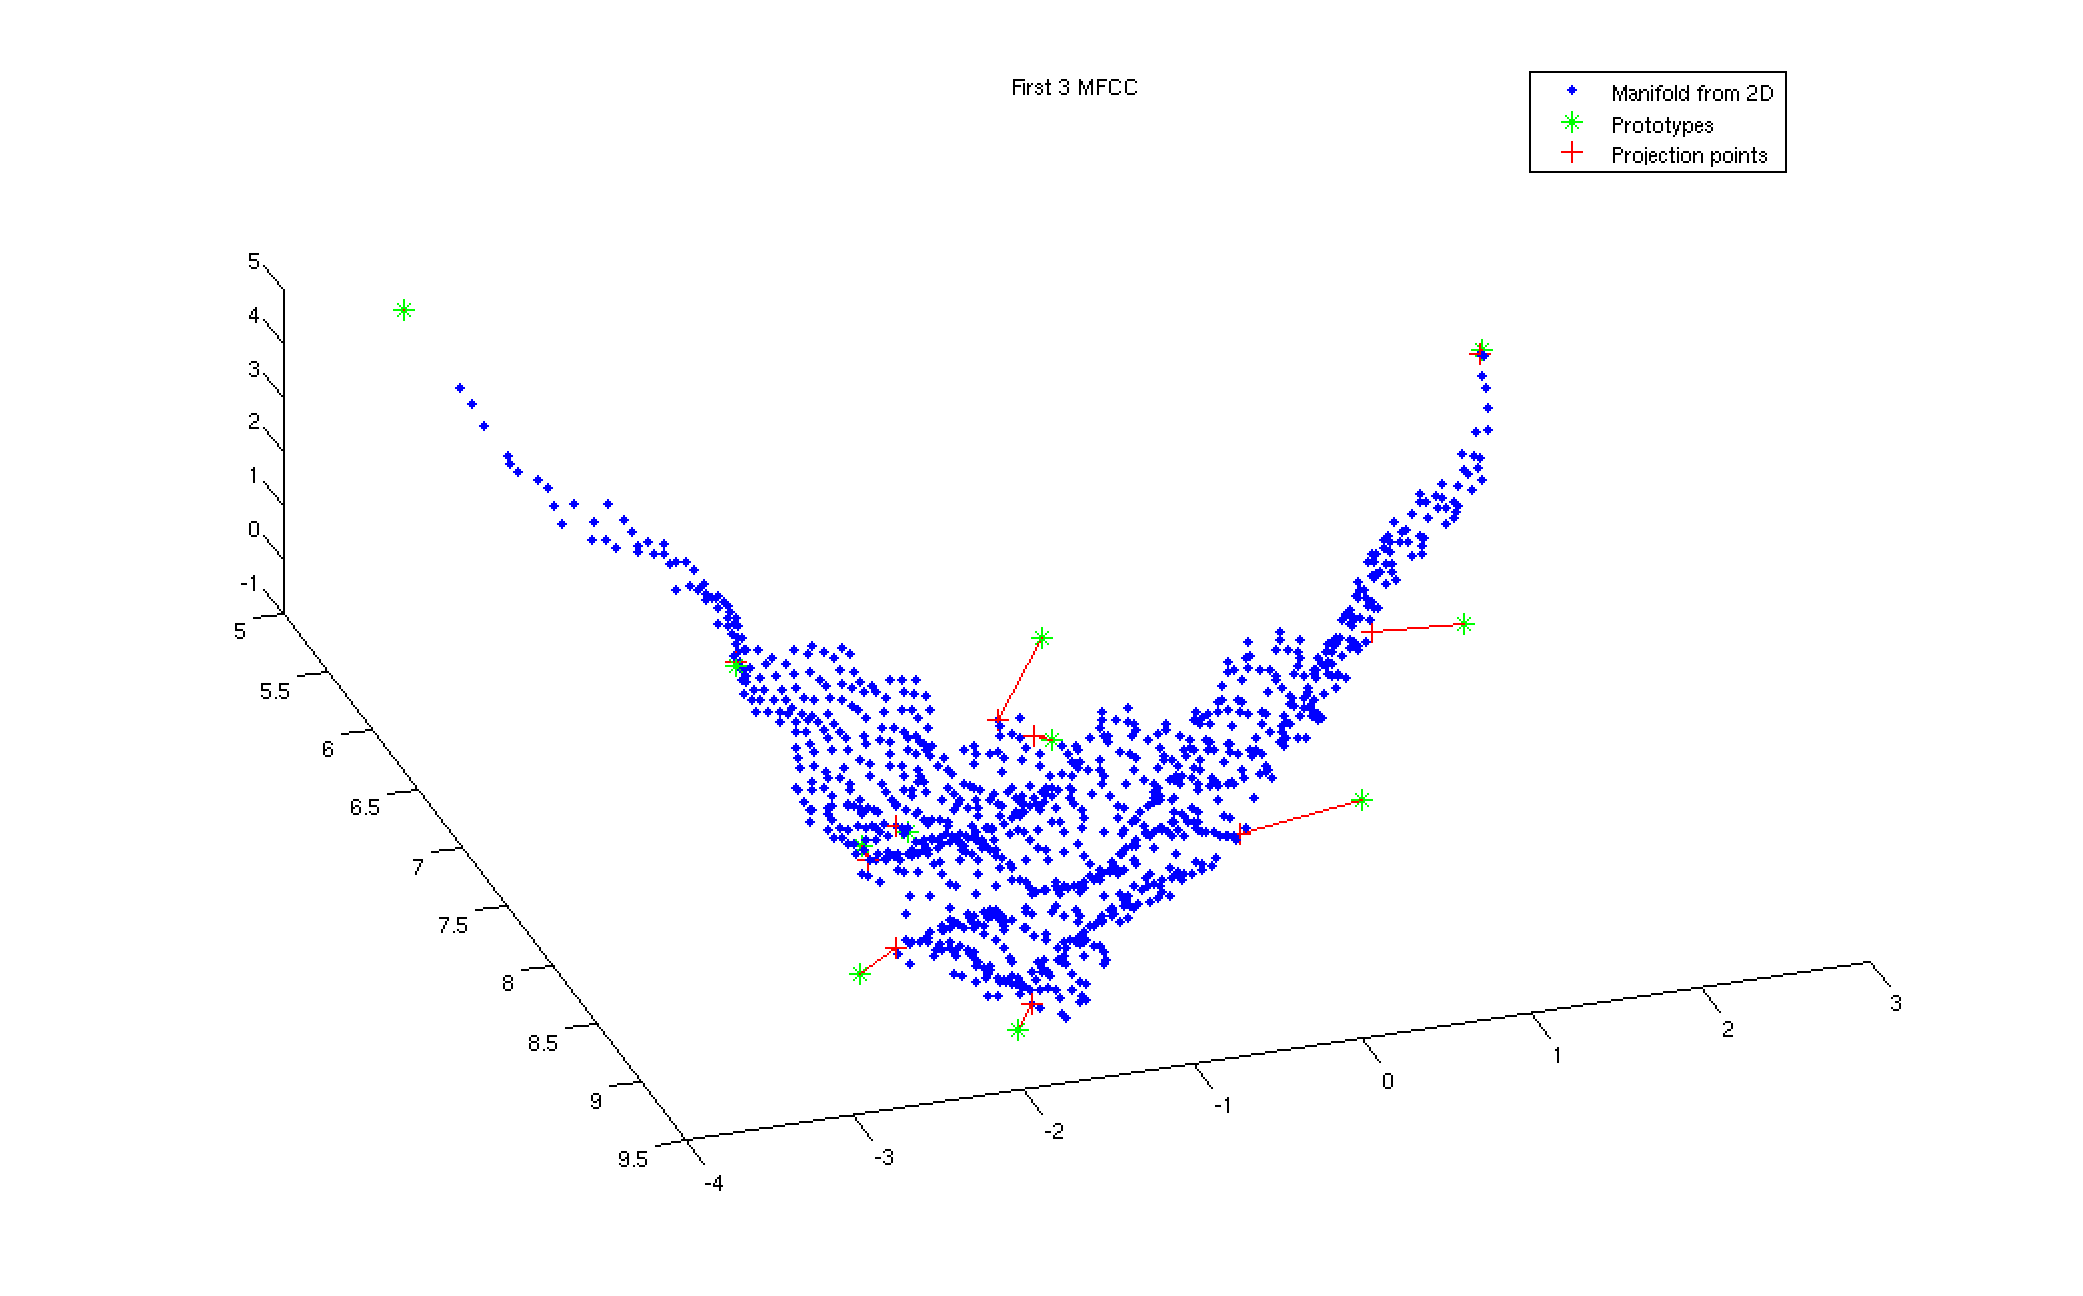
\includegraphics[width=100mm]{include/vowels/images/convex-d2-25-mar}
  \caption{Representation of the approximation error for the chosen
    \emph{VTCalcs} prototypes.}
  \label{fig:convport}
\end{figure}

\begin{figure}[!h]
  \centering
  %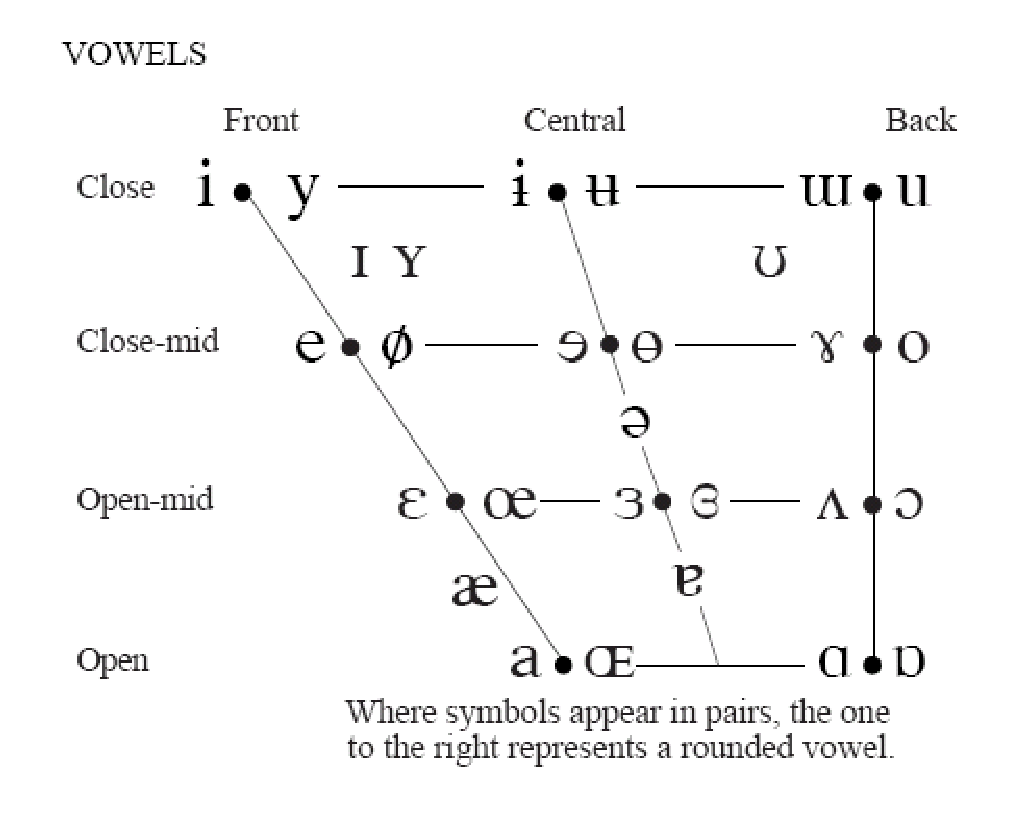
\includegraphics[width=70mm]{include/vowels/images/vowels}
  %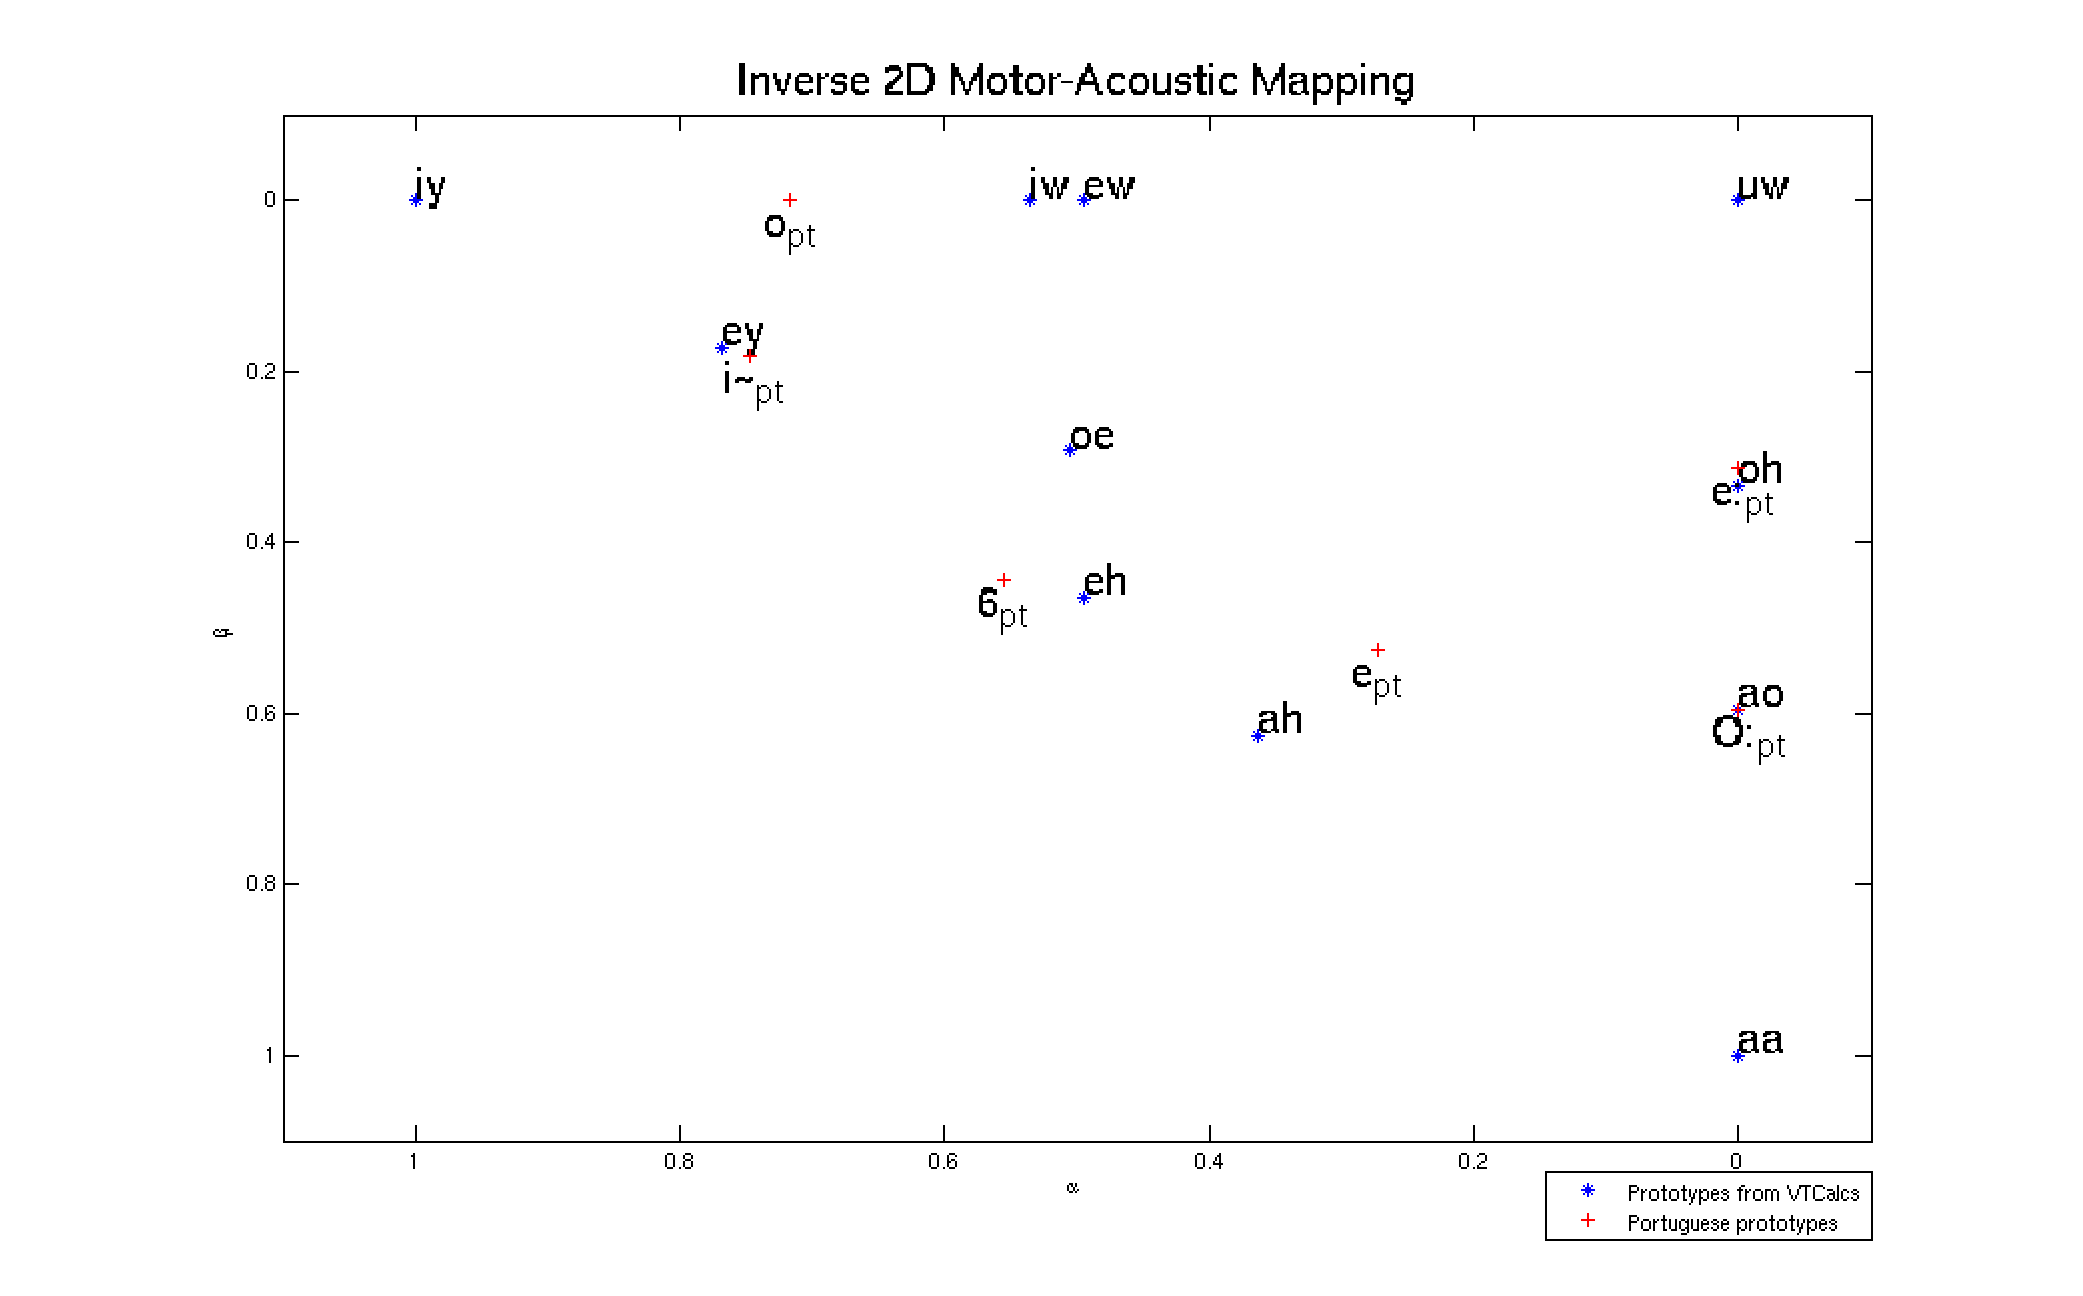
\includegraphics[width=90mm]{include/vowels/images/2dmam}
  \caption{The inverse mapping of the vowel prototypes shows a strong
    correlation between the \emph{height} and \emph{openness} plane
    (top) and the $(\alpha,\beta)$ plane (bottom). The notation for
    the portuguese vowels is SAMPA, except for  \textipa{[e]} (IPA)
    noted as e: and  \textipa{[1]} (IPA) noted as i$\sim$.}
  \label{fig:motormaeda}
\end{figure}

Figure \ref{fig:motormaeda} shows a good approximation between the IPA
Vowel Diagram location for the prototypes and the inverse mapping from
MFCC in acoustic feature space. Although there exists some error, the
ability to construct an invertible mapping between articulatory and
acoustic related spaces in low dimensionality can direct us to improve
normalization procedures on the signals.

\subsection{Conclusions}
The approach is able to generate acoustic signals that represent well
all the vowels produced by the syntesizer.
The proposed model is important by two main reasons:
\begin{itemize}
\item The motor space is two-dimensional, thus can be densely sampled
  with low computational requirements.
  This simplifies creation and representation of the motor acoustic map.
\item The restriction of the synthesizer's function to the proposed
  motor-space is invertible, allowing to map signals back from the
  acoustic to motor coordinates. This will facilitate the utilization
  of learning and classification algorithms.
\end{itemize}
In future work we will quantify the approximation error to human
spoken vowels and evaluate the model's applicability for learning and
recognition. We will also try to improve the basis vowels, so that
they better represent the extremal points in the vocal tract.

Since the acoustic manifold appears to be smooth, we will provide it
with a differential structure and use it for local optimization,
e.g. for guided exploratory learning in imitation tasks. In the long
term we intend to apply the proposed model in the early stages of a
robot learning autonomously to produce and recognize speech. Once the
system learns a good initial model of the motor-audio map using the
low dimensional manifold, it can expand the available degrees of
freedom and refine its production capabilities. As in the ontogenesis
of humans infants, such a developmental strategy is more likely to
succeed than learning from scratch with the whole system's complexity.
\endinput

\bibliographystyle{IEEEbib}
\bibliography{strings,refs}
\begin{thebibliography}{10}
\bibitem{GUNTHER06} Guenther, F.H., Ghosh, S.S., and Tourville, J.A. (2006). Neural modeling and imaging of the cortical interactions underlying syllable production. Brain and Language, 96 (3), pp. 280-301.
\bibitem{liberman85} Liberman, A. and Mattingly, I. (1985), "The motor theory of speech perception revisited", Cognition, 21:1--36. 1985.
\bibitem{gallese96} Gallese, V. and Fadiga, L. and Fogassi, L. and Rizzolatti, G. (1996), "Action Recognition in the Premotor Cortex", Brain, 119:593--609. 1996.
\bibitem{lopes05} Lopes, M. and Santos-Victor, J. (2005), "Visual Learning by Imitation with Motor Representations", IEEE Transaction on Systems Man and Cybernetics -- Part B: Cybernetics, June 2005.
\bibitem{hamzei03} Hamzei, F. and Rijntjes, M. and Dettmers, C. and Glauche, V. and Weiller, C. and Buchel, C. (2003), "The human action recognition system and its relationship to broca's area: and fmri stdy"  Neuroimage, 19:637-644, 2003.
\bibitem{JONES17} Jones, D. (1917), "An English Pronouncing Dictionary", London: Dent, rpt in facsimile in Jones (2002). 17th edn, P. Roach, J. Hartman and J. Setter (eds), Cambridge: CUP, 2006.
\bibitem{IPA} International Phonetic Association. (1999), Handbook of the International Phonetic Association, Cambridge: CUP, 1999. 
\bibitem{TITZE} Titze, I. (1994), Principles of Voice Production, Prentice/Hall
\bibitem{MAEDA}Maeda, S. (1990) ''Compensatory articulation during speech: evidence from the analysis and synthesis of vocal-tract shapes using an articulatory model'' in Speech production and speech 
modelling (W. J. Hardcastle and A. Marchal, eds.), p. 131-149.  Boston: Kluwer Academic 
Publishers.
\bibitem{Davis80} Davis, S. B. and Mermelstein, P. (1980). Comparison of parametric representations for monosyllabic word recognition in continuously spoken sentences. IEEE Transactions on Acoustics, Speech and Signal Processing,  ASSP-28:357-366.
\bibitem{Tenenbaum00} A Global Geometric Framework for Nonlinear Dimensionality Reduction
Joshua B. Tenenbaum, Vin de Silva, and John C. Langford (22 December 2000)
Science 290 (5500), 2319. [DOI: 10.1126/science.290.5500.2319]
\end{thebibliography}

